\documentclass[10pt]{article}
\usepackage[utf8]{inputenc}
\usepackage[english]{babel}
\usepackage{mathrsfs}
\usepackage{graphicx}
\usepackage[euler]{textgreek}
\usepackage{fancyhdr} % For header
\usepackage{mdframed} % for boxes
\usepackage{geometry} % For margins
\usepackage{amsthm} % For theorems
\usepackage{amsmath,amsfonts} % For math
 \geometry{
 a4paper,
 left=.75in,
 right=.75in,
 top=1in,
 }
 \newcommand{\bb}{\mathbb}
 \usepackage{sectsty}
\subsectionfont{\large\underline}
\fancyhf{}
\renewcommand\thesection{}
\renewcommand\thesubsection{}
\fancyhead[L]{\textbf{\leftmark\rightmark}}
\fancyhead[R]{\textbf{Temp Journal }}
%\rhead{\textbf{Temp Journal }}
%\lhead{\textbf{Week}}
\rfoot{Page \thepage}
\pagestyle{fancy}

\theoremstyle{definition}
\newtheorem*{definition}{Definition}
\newtheorem*{example}{Example}
\newtheorem*{theorem}{Theorem}
\newtheorem*{lemma}{Lemma}
\newtheorem*{corollary}{Corrolary}
\setlength{\parskip}{1em}
\setlength{\parindent}{0pt}
\begin{document}

\section{Week 4}

Concern that problems are due to high dimensionality. Focus this week: Filter to one Genus/family/something and repeat.

Start thinking/writing about motivations for needing/wanting to model everything at once instead of running separately.

What dataset to use? Prevalence filter first?
Going to use the 10p filtered dataset and then pick a genus.

Also looking into R ways to resolve phylogenetic tree to genus level.
Potentially group clade? https://yulab-smu.top/treedata-book/chapter6.html

(Needed to add phylogenetic tree to saved rds. )


\subsection{Meeting notes}

Found bug. Ugh. Variance term was incorrect. Check things now.


Try independence,
Try fixed values.
Look at residual matrix (convert to matrix?)
Check that entries match.




\section{Week 5}

Found bug. (In variances). Also note that diriclet variances should be between 0 and 1.

Check with $\gamma = 1$.


Check with $\lambda$


Vocab
\begin{itemize}
  \item $\gamma$: step size
  \item $\rho$: phylogenetic distance scaling
  \item $\omega$: correlation weighting.
  \item $\beta$ estimated parameter values/ coefficients
  \item $\lambda$: diagonal scalar to subtract from Hessian.
\end{itemize}


Tuesday:
Noticed code was getting ugly and hard to navigate. Changed return values to initialize easier by just initilizeing one list that has sub lists inside it.

Note: changed difference (plus convergence criteria) to be sum of square differences between beta between loop.

Wednesday:
Trying on 10p data (by accident oops). Still takes a long time.
Does not have large gaps. Omega approaches 1.


When running on the flavo data, it 'converges' in only 2 iterations. Also check out.

Reminder:
\begin{itemize}
  \item $\omega = 1$ means all weight is compositional structure. If this is the case it doesnt really matter what $\rho $ is
  \item $\omega = 0$ means all weight is phylogenetic structure.
  \item $\rho$ close to 0 means:
  \item $\rho$ large means:
\end{itemize}

Working on a function that outputs all diagnoistics plots. Done. Currently has phi, rho, omega, diffs. Need to add residuals information and beta information. how to visualize? Maybe a line plot with a line for each beta?

Trying 30p dataset which originally had decent values for omega and p.
Quit in 2 iterations. Omega flipped.

\begin{figure}[!htb]
	\centering
	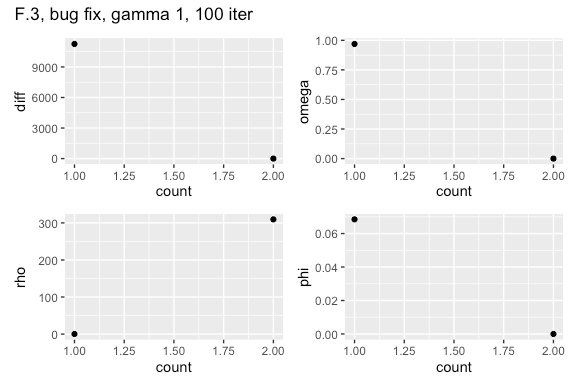
\includegraphics[width=0.35\textwidth]{img/Temp_week_journal-8b0e2d13.png}
	\caption{}
	\label{}
\end{figure}

Next step: step through function with 30p.

\begin{verbatim}
  Browse[2]> beta
 [1]  32.6820041 -35.2771786  -9.3769864   9.8059738  -6.3851386   1.6309199  -9.0146528
 [8]   5.1724875  -7.5425704   2.6913815  -9.4761818   4.5570750  -7.8544924   3.1674555

Browse[2]> as.vector(update)
 [1] -1.252986e-27 -1.252986e-27 -2.654175e-38 -2.654175e-38 -3.051694e-40 -3.051694e-40
 [7] -8.706320e-39 -8.706320e-39 -1.811488e-39 -1.811488e-39 -1.424226e-39 -1.424226e-39
[13] -7.777419e-40 -7.777419e-40 -4.486093e-40 -4.486093e-40 -3.262656e-40 -3.262656e-40
\end{verbatim}

Seems like the 'update' is essentially zero.

Which is because the hessian is essentially zero.
\begin{verbatim}
  Browse[2]> as.vector(hess)
   [1]  -1.000000e-02  -9.860304e-46   1.007366e-76  -2.793269e-79  -2.314020e-64
   [6]  -2.492956e-64   3.834566e-57  -3.314361e-61  -2.560319e-62  -2.595960e-62
  [11]   1.079445e-60  -4.290110e-64  -3.059416e-64  -3.316491e-64   3.727629e-59
  [16]  -2.020623e-63  -6.455299e-63  -6.567340e-63  -1.639493e-49  -1.639493e-49
  [21]   1.620392e-65  -4.701085e-77   1.780107e-59  -2.344796e-60  -3.144451e-56
\end{verbatim}

But estimating equations are also basically zero.
\begin{verbatim}
  Browse[2]> summary(as.vector(esteq))
      Min.    1st Qu.     Median       Mean    3rd Qu.       Max.
-1.253e-29  0.000e+00  0.000e+00  0.000e+00  0.000e+00  1.253e-29
\end{verbatim}

Wondering if this is a step thing? Try with gamma = .1 like before. Seems like a step thing.
With gamma .1:
Some WEIRD behavor with beta plot... Oh, this was some weird result of the beta plotting??? (Had X axis as descrete, but now it is not. )

Quick iteration seems to be a step problem.
But betas are different
For example on the dataset 30p, For gamma = 1 vs gamma = .1

\begin{figure}[!htb]
	\centering
	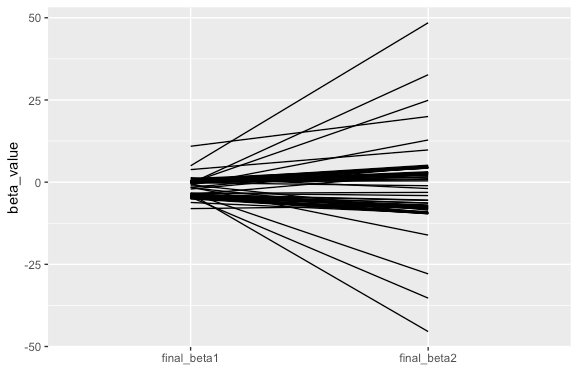
\includegraphics[width=0.35\textwidth]{img/Temp_week_journal-9d4b1490.png}
	\caption{}
	\label{}
\end{figure}




\subsubsection{Independence design}

Try setting R to be the identity matrix.
Only need to change line in \texttt{calculate\_equations} function.

Using values of gamma = .1, 100 iterations.

VERY DIFFERENT...
Here final\_beta2 is independence, final\_beta1 is standard R.
\begin{figure}[!htb]
	\centering
	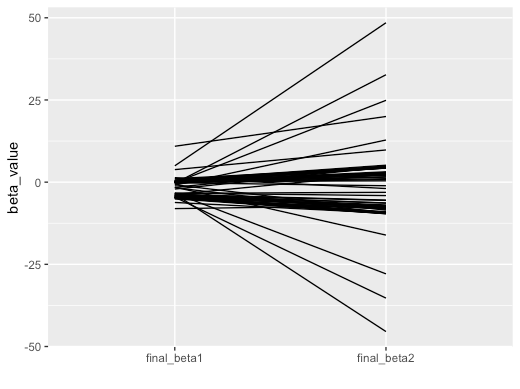
\includegraphics[width=0.35\textwidth]{img/Temp_week_journal-b398c6f5.png}
	\caption{}
	\label{}
\end{figure}

Not sure what I do besides say: they are different!

Try to focus on one thing at once to be able to add git commits.

Shouldnt they be the same though? isnt idea that its just precision that changes? Am confused.


I think the important next step is to test independence design against pre-made functions? like geem.
Can i actually use another package? Since family and link are weird. Look more into GEEM.

... Wait is my link wrong? Since isnt it logit? Or is it because I am linking alpha instead of mu?









\subsection{Meeting}
Bring up:
What was the thing about the metabolomic data?


I explored model running performance after finding the bug. Found that the model "converges" after 2 iterations now, but if step size is reduced, does not. But gives different beta values.


\subsection{Simulations}

Start simulations

Idea that correlation matrix is redundant for dirichlet and we are making it not so



\newpage
\section{Week 6}


Starting simulations!

Need: Example distance matrix. Either from zebrafish, or an example dataset in phyloseq?
Using Global patterns, fecal samples. Randomly select (15?) taxa from more abundant taxa. Extract distance matrix.

Give some beta value. Should be for each taxa. The same? Different? Ask in email.

Split X as even 0s and 1s.
Do i set an intercept?? No?

Set omega, set rho.

Calculate alpha as $\log \alpha = X \beta$.

Calculate $R$ from $\alpha, \rho, D, \omega$.

Simulate $y \sim N(\alpha/\alpha_0, R)$
Which shares the same mean and covariance as the model.
but Doesnt have the same variance? or does it?

Also R is covariance matrix not variance? So there is a $\sigma^2$ value?

Stop getting confused about variance/ covariance/ correlation.

Standardize. Ask? Calculate sum above zero etc, proportion...
Report.

UMM I think the get\_dirichlet\_cor function is the CoVARIANCE. But for R i want the VARIANCE?? Nope it is ok. Acutally calculated the correlation and it is correct. The numerator looks funny.. Wait... actually there is missing a square root! Nope it is there in the code. Everything is fine.

\begin{align*}
  Cor_D &= \frac{Cov}{\sqrt V_i \sqrt V_j}\\
  &= -\frac{\alpha_i\alpha_j}{\alpha_0^2 (\alpha_0 + 1)} \sqrt{\frac{\alpha_0^2 (\alpha_0 + 1)}{\alpha_i(\alpha_0 - \alpha_i)}} \sqrt{\frac{\alpha_0^2 (\alpha_0 + 1)}{\alpha_j(\alpha_0 - \alpha_j)}}\\
  &= - \sqrt{\frac{\alpha_i \alpha_j}{(\alpha_0 - \alpha_i)(\alpha_0 - \alpha_j )}}
\end{align*}

NOTE! in rho omega fun, changed matrix to byrow = T. bug? test.

Hmm. Does this matter? it didnt change the beta values at all..

Final beta results
\begin{verbatim}
  [[50]]
 [1]   4.5424926  -2.3861832  -6.2525309   3.2004029   0.5698044  -3.6470294  -5.9934911
 [8]   3.1636061   5.8906071  -8.1679282  -6.1703515   4.7639107  -1.6003967   0.5118927
[15]  -6.1924151   4.6084286  -7.9448292 -10.0329420  -6.3725543   4.8713606   2.3284297
[22]  -3.8093811  -6.1630714   4.7997512   1.6008044  -3.3514829  -6.2586418   4.6867781
[29]  -2.6127452   0.7888159
\end{verbatim}

Want


umm still getting infinities with this data..



\subsection{Meeting}
Run with only dirichlet instead (set omega = 1)

Make sure GEE runs with just dirichlet data.
Try also with true correltion/covariance matrix V just to get right betas.

Seems like intercept term did not initialize well. Just have it be 0.

CHECK that matrix colsumns has correlctly byrow = T or byrow = F in it! make sure it is right.


\newpage

\section{Week 7}

Trying to do better with version control. Did some reorganizing. See todo and commits

Want to work though to make sure indeces of everything are what I'm intending.

Do I make everything a dataframe with the intended index?

So do we allow an intercept even when simulated with no intecept? Yes?



\subsection{Dirichlet simulation}
Found one issue that might be why it wasnt working in the meeting. Alphas were being generated for each p not each n.

Comment out the wRrho_res function in meeting.

Code in a way to only have dirichlet correlation.

Stepping through function:
n = 100, p = 15, phi = 1, q = 2 (adds intercept), rho = 5 (doesnt matter since omega = 1 - all dirichlet)


Ok, ran through but still didnt work... Also the difference was (increasing???)

Now step through. Since we know the 'true' alpha values, we can compare.

Noticed update beta step still needed R inv. changed.

iter 0: all 30 beta values 0.

Seems like first step always has a better beta value. Do I have a wrong minus sign? ugh.

\end{document}
